%Use one of the two documentclass lines depending on aspect ratio needed
% for 4x3 aspect ratio slides
%\documentclass{beamer}
%for 16x9 (modern wide screen) aspect ratio slides
\documentclass[aspectratio=169]{beamer}

% Oxford Maths theming
\usetheme{oxfordmaths}

% Set author etc info
\title[Automated Goal-Based Adaptivity for Time-Dependent PDEs] %short version of title for slide footer
{Automated Goal-Based Adaptivity for Time-Dependent PDEs} %full title for titlepage
\author{Yue Wu \\ Supervisor: Prof.\ Patrick Farrell}
\institute{Mathematical Institute\\University of Oxford}
\date[5 June 2026]  %short date for slide footer
{MSc Dissertation Presentation, June 2026} %main date for title page,
                        %can overload it to show say 'Conference X, Date Y'

% Macros
\newcommand{\R}{\mathbb{R}}
\newcommand{\Vh}{V_h}
\newcommand{\Vhe}{V_h^{(2)}}
\newcommand{\inner}[2]{\langle #1, #2 \rangle}

% block styles
\setbeamertemplate{blocks}[rounded][shadow=false]

\setbeamercolor{block title example}{fg=white,bg=green!60!black}
\setbeamercolor{block body example}{fg=black,bg=green!7}
\setbeamerfont{block title example}{series=\bfseries}

\setbeamercolor{block title alerted}{fg=white,bg=red!70!black}
\setbeamercolor{block body alerted}{fg=black,bg=red!7}
\setbeamerfont{block title alerted}{series=\bfseries}

\newcommand{\redu}{\alt<3>{\textcolor{red}{u}}{u}}
\newcommand{\redz}{\alt<3>{\textcolor{red}{z}}{z}}

% technology changes life
\usepackage{tikz}
\usetikzlibrary{arrows.meta, positioning, fit, calc}


% --- colors ---
\definecolor{OxfordBlue}{RGB}{0,33,71}
\definecolor{TextGrey}{RGB}{84,92,105}
\definecolor{TimelineDone}{RGB}{76,160,88}
\definecolor{TimelineTheory}{RGB}{210,77,73}
\definecolor{TimelineModel}{RGB}{54,127,199}
\definecolor{TimelineVerify}{RGB}{235,154,52}
\definecolor{TimelineWrite}{RGB}{119,90,178}

% --- project plan data ---
\newcommand{\Ntasks}{7}




\begin{document}


% --- Title ---
\begin{frame}[plain]
    \titlepage
\end{frame}


% --- Outline ---
\begin{frame}{Outline}
    \tableofcontents[hideallsubsections]
\end{frame}


% --- Motivation 1 ---
\section{Motivation and Goal Functionals}
\begin{frame}{Motivation}

In many applications, we do not need the full solution.
\vspace{0.3em}

\pause
We care about a specific \textbf{quantity of interest}:
\[
    J : V \to \mathbb{R}.
\]
\end{frame}


% --- Motivation 2 ---
\begin{frame}{Goal Functionals}
\vspace{-1em}
\begin{overlayarea}{\textwidth}{10cm}

\only<1>{
\begin{exampleblock}{Example: fusion reactor}
    \small
    Find $\phi \in V$ and $k_{\mathrm{eff}} \in \mathbb{R}$ such that
    \[
        A\phi = \frac{1}{k_{\mathrm{eff}}}B\phi.
    \]
    A natural goal functional is
    \[
        J(\phi) = (k_{\mathrm{eff}}-1)^2.
    \]
\end{exampleblock}
\vspace{0.5em}
\centering
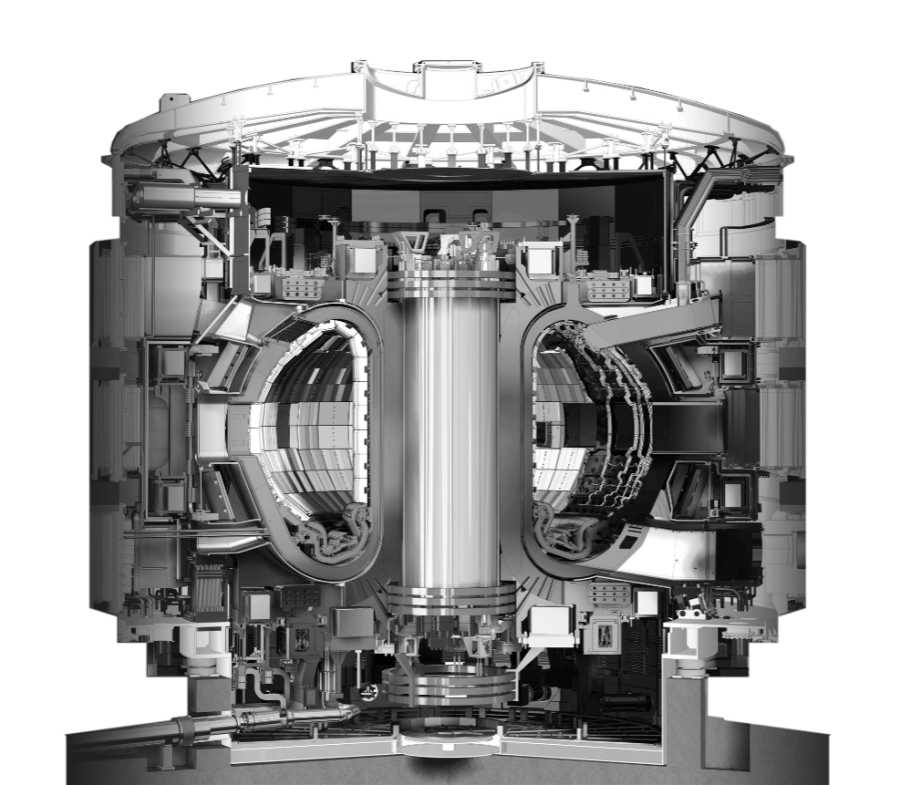
\includegraphics[height=3cm]{fusion-reactor.png}
}

\only<2>{
\begin{exampleblock}{Example: flow past a wing}
    \small
    Let $(u,p)$ solve the incompressible Navier--Stokes equations in $\Omega$:
    \[
        -\nu \Delta u + (u\cdot\nabla)u + \nabla p = f,
        \qquad
        \nabla\cdot u = 0.
    \]
    \vspace{-0.5em}
    A natural goal functional is the drag force:
    \[
        J(u,p)
        =
        \int_{\Gamma_{\mathrm{wing}}}
        \sigma(u,p)n \cdot e_x \, ds.
    \]
\end{exampleblock}

\vspace{0.4em}
\centering
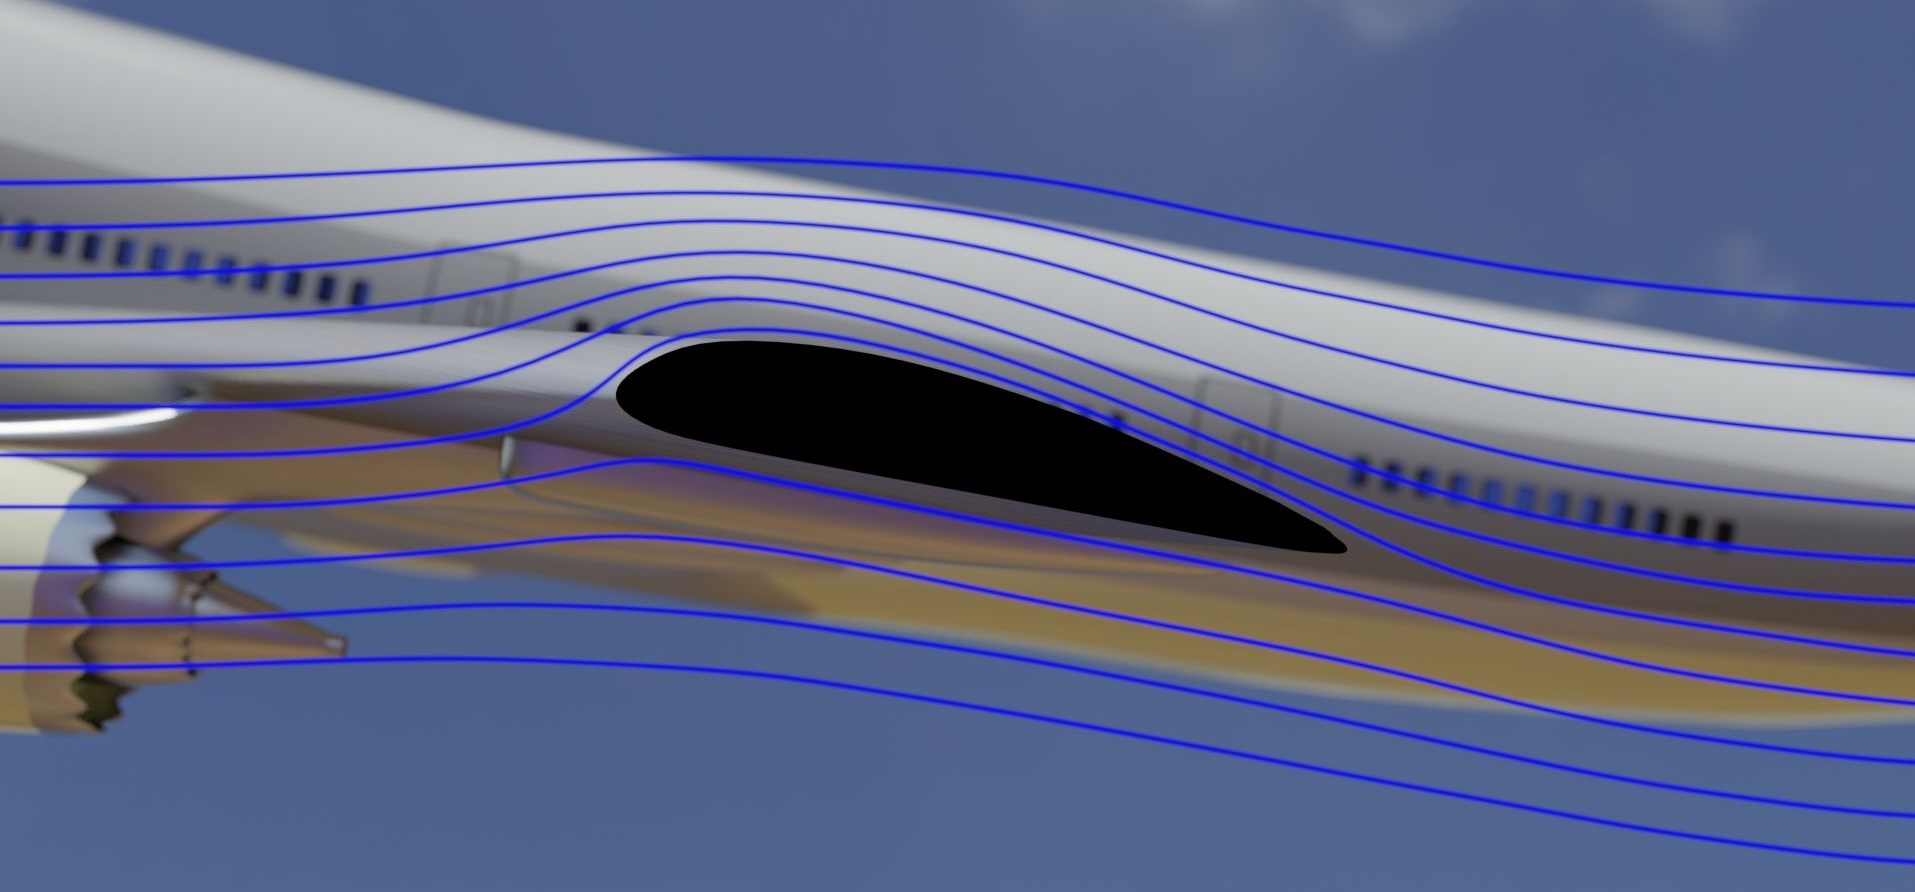
\includegraphics[height=2.5cm]{flow-past-wing.jpg}
}

\end{overlayarea}

\end{frame}


% --- Problem Formulation ---
\section{Problem Formulation}
\begin{frame}{Problem Formulation}
\textbf{Primal problem.} Find the exact solution $u \in V$ such that 
% \vspace{-0.5em}
$$\mathcal{A}(u)(v) = 0 \quad \forall v \in V.$$
% \vspace{-0.5em}
Here $\mathcal{A}$ incorporates both spatial and temporal operators.
\vspace{0.5em}
\pause

\textbf{Finite Element discretisation.} Find the discrete approximation $u_h \in V_h$ s.t.
% \vspace{-0.5em}
$$\mathcal{A}(u_h)(v_h) = 0 \quad \forall v_h \in V_h.$$
\vspace{-1em}
\pause

\textbf{Goal functional.} In practice, we are interested in a specific quantity of interest
% \vspace{-0.5em}
$$J : V \to \mathbb{R}.$$
\vspace{-1em}
\pause

\textbf{Objective.} Estimate the goal error
$$\eta \approx |J(u) - J(u_h)|,$$
and drive adaptivity so that it stays below a prescribed tolerance $\eta < $ TOL.
\end{frame}


% --- DWR 1 ---
\section{Dual-Weighted Residual Method}
\begin{frame}[t]{DWR: Adjoint Problem and Error Identity}

\begin{columns}[T,onlytextwidth]
    \begin{column}{0.78\textwidth}
        \small

        \textbf{Adjoint problem.}
        Find \(z \in V\) such that
        \[
            \mathcal{A}'(u)(\phi, z) = J'(u)(\phi)
            \qquad \forall \phi \in V.
        \]

        \vspace{0.5em}

        \only<2->{
        \textbf{Error identity.}
        For arbitrary approximations \(\tilde u \in U\) and \(\tilde z \in V\),
        \[
        J(u)-J(\tilde u)
        =
        \frac12\Big(
            \rho(\tilde u)(z-\tilde z)
            +
            \rho^*(\tilde u,\tilde z)(u-\tilde u)
        \Big)
        - \rho(\tilde u)(\tilde z)
        + \mathcal{R}^{(3)}.
        \]
        }

        \vspace{0.4em}

        \only<3->{
        \textbf{Residual terms.}
        \[
            \rho(\tilde u)(\cdot) := -\mathcal{A}(\tilde u)(\cdot),
            \qquad
            \rho^*(\tilde u,\tilde z)(\cdot)
            := J'(\tilde u)(\cdot)-\mathcal{A}'(\tilde u)(\cdot,\tilde z).
        \]

        \vspace{0.3em}
        The remainder \(\mathcal{R}^{(3)}\) contains higher-order terms.
        }
    \end{column}

    \begin{column}{0.20\textwidth}
        \centering

        \only<2->{
        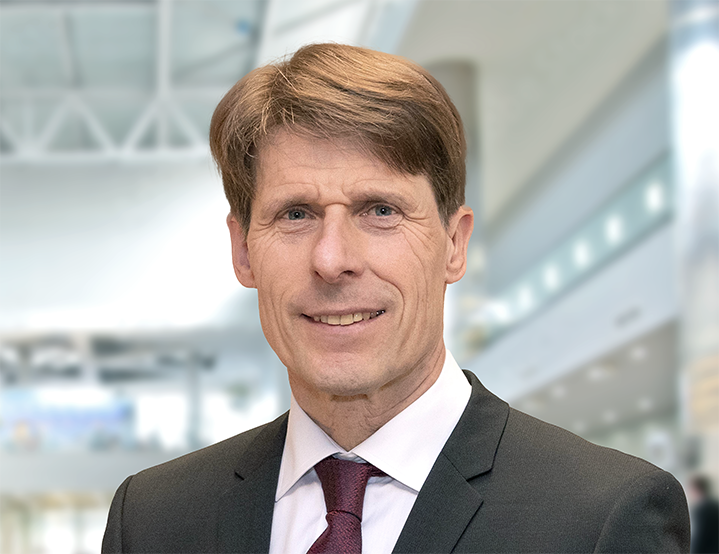
\includegraphics[width=\linewidth]{Roland-Becker.png}

        \vspace{0.2em}
        {\scriptsize Roland Becker}
        }

        \vspace{1.0em}

        \only<2->{
        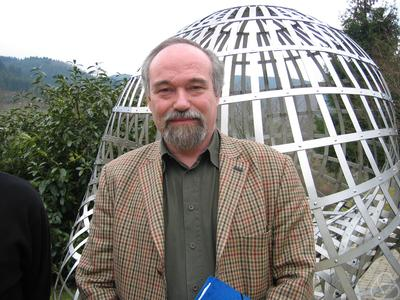
\includegraphics[width=\linewidth]{Rolf-Rannacher.jpeg}

        \vspace{0.2em}
        {\scriptsize Rolf Rannacher}
        }
    \end{column}
\end{columns}

\end{frame}


% --- DWR 2 ---
\begin{frame}[t]{DWR: Error Identity and Practical Approximation}

\[
J(\redu)-J(\tilde u)
=
\frac12\Big(
\rho(\tilde u)(\redz-\tilde z)
+
\rho^*(\tilde u,\tilde z)(\redu-\tilde u)
\Big)
-\rho(\tilde u)(\tilde z)
+\mathcal{R}^{(3)}.
\]

\vspace{0.4em}

\onslide<2->{
\begin{exampleblock}{Good news}
The identity does not contain unknown constants.
\end{exampleblock}
}
\vspace{0.5em}

\onslide<3->{
\begin{alertblock}{Bad news}
The exact solution terms \(\redu\) and \(\redz\) are unknown, so the formula is not directly computable.
\end{alertblock}
}
\vspace{0.5em}

\onslide<4->{
\textbf{To make DWR practical: enriched spaces.}}

\end{frame}



% --- DWR 3 ---
\begin{frame}[t]{DWR: Enriched Spaces and Effectivity Index}

We solve on enriched spaces
\[
u_h^{(2)} \in U_h^{(2)}, \qquad z_h^{(2)} \in V_h^{(2)},
\qquad
U_h \subset U_h^{(2)} \subset U,
\qquad
V_h \subset V_h^{(2)} \subset V,
\]
so that \[ J(u)-J(\tilde u) = \underbrace{J(u)-J(u_h^{(2)})}_{\text{small under assumption}} + \underbrace{J(u_h^{(2)})-J(\tilde u)}_{\text{error identity}} \]

\vspace{0.6em}
\pause

The \textbf{effectivity index}
\[
I_{\mathrm{eff}} := \frac{|\eta|}{|J(u)-J(u_h)|}
\]
measures how well the estimator matches the true goal error.

\end{frame}


\begin{frame}[t]{DWR: a Stationary Example}
\begin{columns}[T,onlytextwidth]
% ---------------- Left ----------------
\begin{column}{0.6\textwidth}
\begin{exampleblock}{Example: Poisson problem}
\small
Find $u:\overline{\Omega}\to\mathbb{R}$ such that
\[
-\Delta u = f \quad \text{in } \Omega=(0,1)^2,
\qquad
u=0 \quad \text{on } \partial\Omega.
\]
Goal functional:
\[
J(u)=u(0.5,0.5).
\]
\end{exampleblock}
\vspace{1em}
The DWR estimator is asymptotically effective:
\[
I_{\mathrm{eff}}
=\frac{|\eta|}{|J(u_{\mathrm{ref}})-J(u_h)|}
\approx 1
\quad \text{after refinement.}
\]
\end{column}

\pause
% ---------------- Right ----------------
\begin{column}{0.38\textwidth}
\centering
\small
\vspace{3em}
\textbf{Effectivity on refined meshes}

\vspace{0.8em}

\renewcommand{\arraystretch}{1.15}
\begin{tabular}{c c}
\hline
Dofs & $I_{\mathrm{eff}}$ \\
\hline
18    & 9.98e-01 \\
50    & 1.00e+00 \\
162   & 1.00e+00 \\
482   & 1.03e+00 \\
1794 & 1.02e+00 \\
\hline
\end{tabular}

\vspace{0.8em}
{\scriptsize Becker \& Rannacher, Table 2.}
\end{column}
\end{columns}

\end{frame}


% --- Algorithm ---
\section{Goal-based Adaptivity}
\begin{frame}[t]{Goal-based Adaptivity for Time-dependent Problem}

A DWR-driven adaptive workflow is:

\vspace{0.8em}

\begin{center}
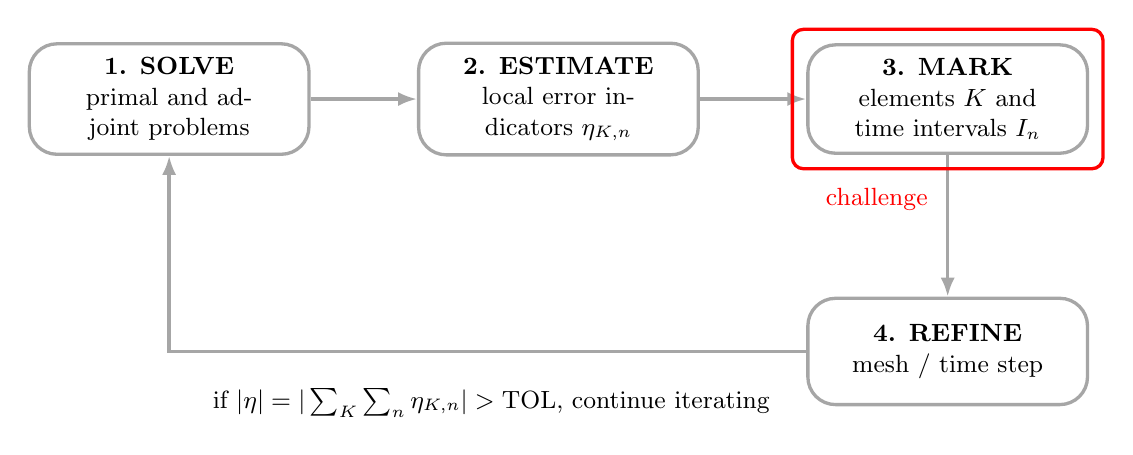
\begin{tikzpicture}[
    font=\small,
    box/.style={
        draw=gray!70,
        very thick,
        rounded corners=10pt,
        align=center,
        minimum height=1.35cm,
        inner sep=5pt,
        text width=3.2cm,
        fill=white
    },
    arrow/.style={-{Latex[length=2.4mm]}, very thick, draw=gray!70}
]

\node[box] (solve) {\textbf{1. SOLVE}\\ primal and adjoint problems};
\node[box, right=1.35cm of solve] (estimate) {\textbf{2. ESTIMATE}\\ local error indicators $\eta_{K,n}$};
\node[box, right=1.35cm of estimate] (mark) {\textbf{3. MARK}\\ elements $K$ and time intervals $I_n$};

\node[box, below=1.8cm of mark] (refine) {\textbf{4. REFINE}\\ mesh / time step};

\draw[arrow] (solve) -- (estimate);
\draw[arrow] (estimate) -- (mark);
\draw[arrow] (mark) -- (refine);

\draw[arrow] (refine.west) -- ++(-8,0) -| (solve.south);

\node[font=\small] at ($(refine.west)+(-4,-0.65)$)
{if $|\eta| = |\sum_K \sum_n \eta_{K,n}| > \mathrm{TOL}$, continue iterating};


% challenge!!
\only<2->{
    \node[draw=red, very thick, rounded corners=4pt, fit=(mark), inner sep=5pt] {};
    \node[red, below=3mm of mark, xshift=-9mm] {challenge};
}

\end{tikzpicture}
\end{center}

\end{frame}



% --- Implementation Plan ---
\section{Project Timeline}
% \begin{frame}{Project Plan}
%     \begin{itemize}
%         \item \textbf{Tools:} Firedrake for FEM assembly, Irksome for time discretisation, and (?)Pyadjoint for automatic adjoints.
%         \item \textbf{Plan:} verify adjoints for time-dependent problems, implement linear DWR estimators manually, then automate the workflow.
%         \item \textit{(Aspirational Extension)} extend the approach to nonlinear problems.
%         \item \textbf{Outcome:} a Firedrake-based tool for goal-oriented adaptivity in time-dependent PDEs.
%     \end{itemize}
% \end{frame}
\begin{frame}{Project Timeline}
\scriptsize

\begin{columns}[T,onlytextwidth]
% ---------------- Left column ----------------
\begin{column}{0.42\textwidth}
\vspace{0.2cm}
\textbf{\textcolor{OxfordBlue}{Completed work}}
\vspace{0.05cm}

\noindent\textbf{\textcolor{OxfordBlue}{1}}\hspace{0.07cm}
\tikz[baseline=-0.45ex]\draw[fill=TimelineDone, draw=OxfordBlue, line width=0.35pt]
(0,0) rectangle (0.17,0.17);
\hspace{0.08cm}\begin{minipage}[t]{4.20cm}\raggedright
Literature review.
\end{minipage}\par\vspace{0.03cm}

\noindent\textbf{\textcolor{OxfordBlue}{2}}\hspace{0.07cm}
\tikz[baseline=-0.45ex]\draw[fill=TimelineDone, draw=OxfordBlue, line width=0.35pt]
(0,0) rectangle (0.17,0.17);
\hspace{0.08cm}\begin{minipage}[t]{4.20cm}\raggedright
Reproduce the full workflow on the 2D heat equation.
\end{minipage}\par\vspace{0.03cm}

\vspace{0.28cm}
\textbf{\textcolor{OxfordBlue}{Planned work}}
\vspace{0.05cm}

\noindent\textbf{\textcolor{OxfordBlue}{3}}\hspace{0.07cm}
\tikz[baseline=-0.45ex]\draw[fill=TimelineTheory, draw=OxfordBlue, line width=0.35pt]
(0,0) rectangle (0.17,0.17);
\hspace{0.08cm}\begin{minipage}[t]{4.20cm}\raggedright
Verify the adjoint formulation for time-dependent problems.
\end{minipage}\par\vspace{0.03cm}

\noindent\textbf{\textcolor{OxfordBlue}{4}}\hspace{0.07cm}
\tikz[baseline=-0.45ex]\draw[fill=TimelineModel, draw=OxfordBlue, line width=0.35pt]
(0,0) rectangle (0.17,0.17);
\hspace{0.08cm}\begin{minipage}[t]{4.20cm}\raggedright
Implement linear DWR estimators manually.
\end{minipage}\par\vspace{0.03cm}

\noindent\textbf{\textcolor{OxfordBlue}{5}}\hspace{0.07cm}
\tikz[baseline=-0.45ex]\draw[fill=TimelineVerify, draw=OxfordBlue, line width=0.35pt]
(0,0) rectangle (0.17,0.17);
\hspace{0.08cm}\begin{minipage}[t]{4.20cm}\raggedright
Automate the workflow.
\end{minipage}\par\vspace{0.03cm}

\noindent\textbf{\textcolor{OxfordBlue}{6}}\hspace{0.07cm}
\tikz[baseline=-0.45ex]\draw[fill=TimelineWrite, draw=OxfordBlue, line width=0.35pt]
(0,0) rectangle (0.17,0.17);
\hspace{0.08cm}\begin{minipage}[t]{4.20cm}\raggedright
Build a Firedrake-based prototype for goal-oriented adaptivity.
\end{minipage}\par\vspace{0.03cm}

\noindent\textbf{\textcolor{OxfordBlue}{7}}\hspace{0.07cm}
\tikz[baseline=-0.45ex]\draw[fill=TimelineWrite, draw=OxfordBlue, line width=0.35pt]
(0,0) rectangle (0.17,0.17);
\hspace{0.08cm}\begin{minipage}[t]{4.20cm}\raggedright
Write up the thesis.
\end{minipage}\par\vspace{0.03cm}

\vspace{0.24cm}
\textbf{\textcolor{OxfordBlue}{Aspirational extension}}

\vspace{0.03cm}
\begin{minipage}[t]{4.20cm}\raggedright
Extend the approach to nonlinear problems if time permits.
\end{minipage}
\end{column}

% ---------------- Right column ----------------
\begin{column}{0.56\textwidth}
\begin{center}
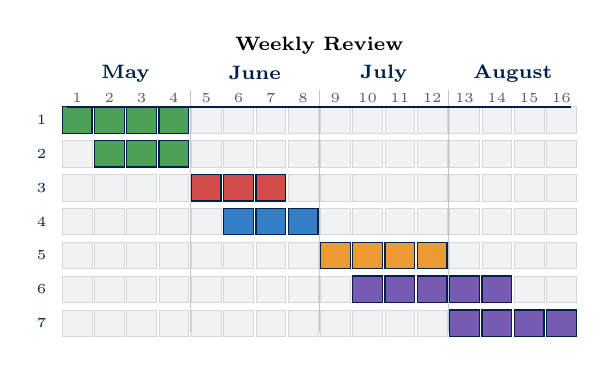
\begin{tikzpicture}[
    x=0.41cm,
    y=0.43cm,
    font=\tiny
]
\node[font=\scriptsize\bfseries] at (8.5,1.10) {Weekly Review};

% Month headers
\foreach \x/\lab in {2.5/May,6.5/June,10.5/July,14.5/August}{
  \node[font=\scriptsize\bfseries, text=OxfordBlue] at (\x,0.28) {\lab};
}

% Month dividers
\foreach \x in {4.5,8.5,12.5}{
  \draw[TextGrey!35] (\x,-0.20) -- (\x,-7.35);
}

% Week numbers
\foreach \w in {1,...,16}{
  \node[text=TextGrey] at (\w,-0.45) {\w};
}

% Row numbers and background grid
\foreach \n in {1,...,\Ntasks}{
  \pgfmathsetmacro{\y}{-1.10 - (\n-1)*1.0}
  \node[anchor=east, font=\tiny, text=OxfordBlue] at (0.35,\y) {\n};

  \foreach \w in {1,...,16}{
    \draw[fill=TextGrey!8, draw=TextGrey!25, line width=0.25pt]
      (\w-0.46,\y-0.39) rectangle (\w+0.46,\y+0.39);
  }
}

% Task 1: literature review
\foreach \w in {1,2,3,4}{
  \draw[fill=TimelineDone, draw=OxfordBlue, line width=0.45pt]
    (\w-0.46,-1.49) rectangle (\w+0.46,-0.71);
}

% Task 2: heat equation reproduction
\foreach \w in {2,3,4}{
  \draw[fill=TimelineDone, draw=OxfordBlue, line width=0.45pt]
    (\w-0.46,-2.49) rectangle (\w+0.46,-1.71);
}

% Task 3: adjoint verification
\foreach \w in {5,6,7}{
  \draw[fill=TimelineTheory, draw=OxfordBlue, line width=0.45pt]
    (\w-0.46,-3.49) rectangle (\w+0.46,-2.71);
}

% Task 4: manual DWR estimators
\foreach \w in {6,7,8}{
  \draw[fill=TimelineModel, draw=OxfordBlue, line width=0.45pt]
    (\w-0.46,-4.49) rectangle (\w+0.46,-3.71);
}

% Task 5: automation
\foreach \w in {9,10,11,12}{
  \draw[fill=TimelineVerify, draw=OxfordBlue, line width=0.45pt]
    (\w-0.46,-5.49) rectangle (\w+0.46,-4.71);
}

% Task 6: Firedrake prototype
\foreach \w in {10,11,12,13,14}{
  \draw[fill=TimelineWrite, draw=OxfordBlue, line width=0.45pt]
    (\w-0.46,-6.49) rectangle (\w+0.46,-5.71);
}

% Task 7: thesis writing
\foreach \w in {13,14,15,16}{
  \draw[fill=TimelineWrite, draw=OxfordBlue, line width=0.45pt]
    (\w-0.46,-7.49) rectangle (\w+0.46,-6.71);
}

% top baseline
\draw[OxfordBlue, thick] (0.70,-0.72) -- (16.30,-0.72);

\end{tikzpicture}
\end{center}
\end{column}
\end{columns}

\end{frame}




% !! Reference and Thank you page !!








\end{document}
